\documentclass{beamer}
\usetheme{metropolis}           % Use metropolis theme
\usepackage[utf8]{inputenc}
\usepackage[spanish]{babel}
\title{Estudio demográfico de las grandes empresas en España}
\date{\today}
\author{Francisco Luque Sánchez\\
María del Mar Ruiz Martín}
\institute{Ingeniería, empresa y sociedad}

\begin{document}

\maketitle

\section{Grandes empresas en España}

\begin{frame}{Evolución anual}
  \begin{figure}[H]
    \centering
    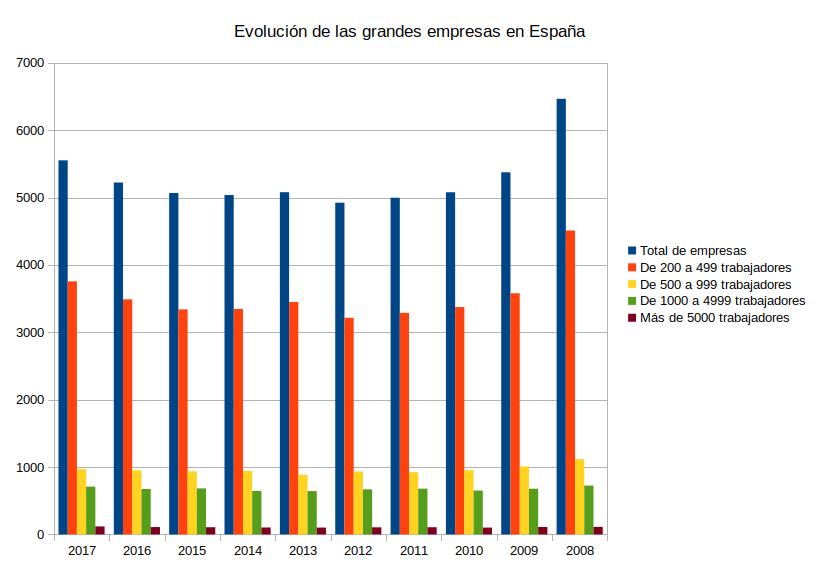
\includegraphics[width=.8\textwidth]{../graficos/barras_evolucion_anual}
    \caption{Evolución del tamaño de las empresas en España}
  \end{figure}
\end{frame}

\begin{frame}{Distribución geográfica}
  \begin{figure}[H]
    \centering
    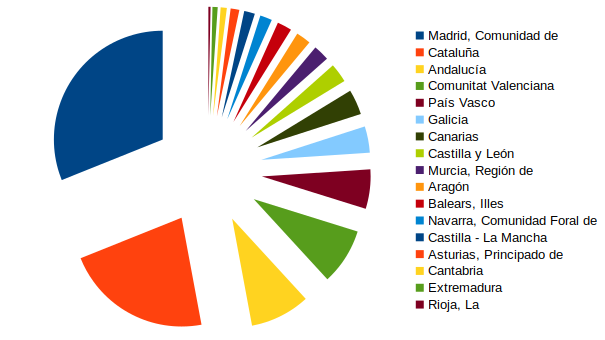
\includegraphics[width=.9\textwidth]{../graficos/sectores_comunidades}
    \caption{Distribución de las grandes empresas en el territorio
      español}
  \end{figure}
\end{frame}

\section{Estadísticas de empresas filiales en el extranjero}

\begin{frame}{Empresas filiales}
  \begin{figure}[H]
    \centering
    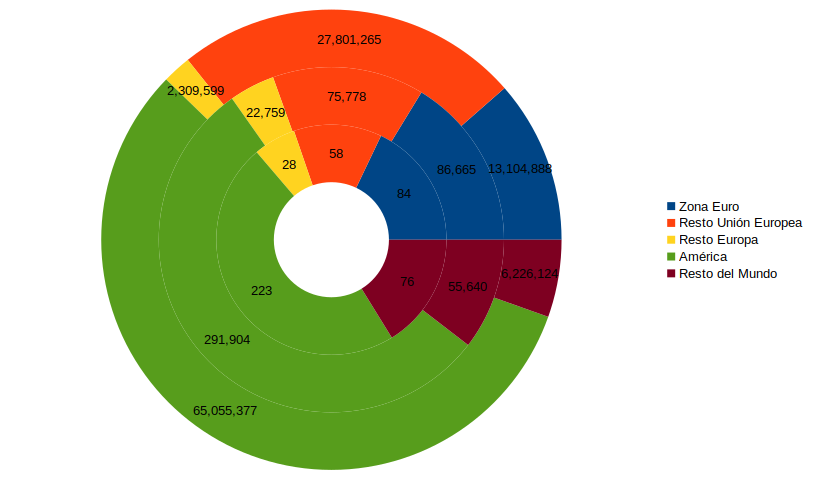
\includegraphics[width=\textwidth]{../graficos/sectores_filiales}
    \caption{Distribución de filiales de las empresas españolas en el
      extranjero}
  \end{figure}
\end{frame}

\section{Productividad}

\begin{frame}{Productividad en el sector servicios}
\begin{figure}[H]
  \centering
  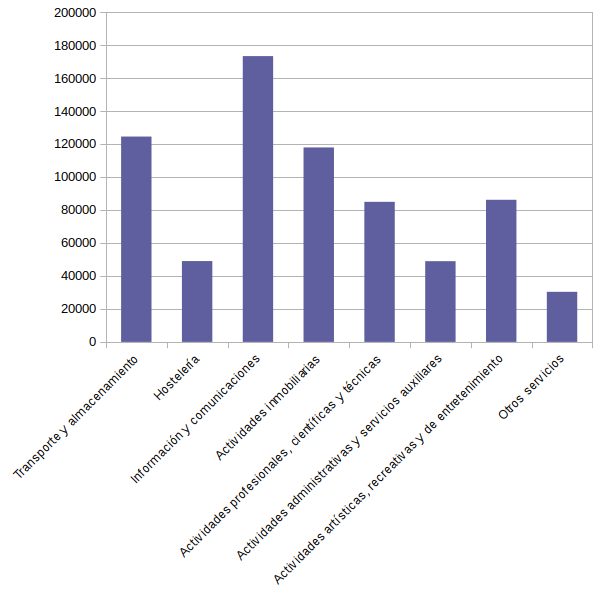
\includegraphics[width=.6\textwidth]{../graficos/barras_productividad_servicios}
  \caption{Productividad de los trabajadores dentro del sector
    servicios}
\end{figure}
\end{frame}

\begin{frame}{Productividad y empleabilidad por sectores}
\begin{figure}[H]
  \centering
  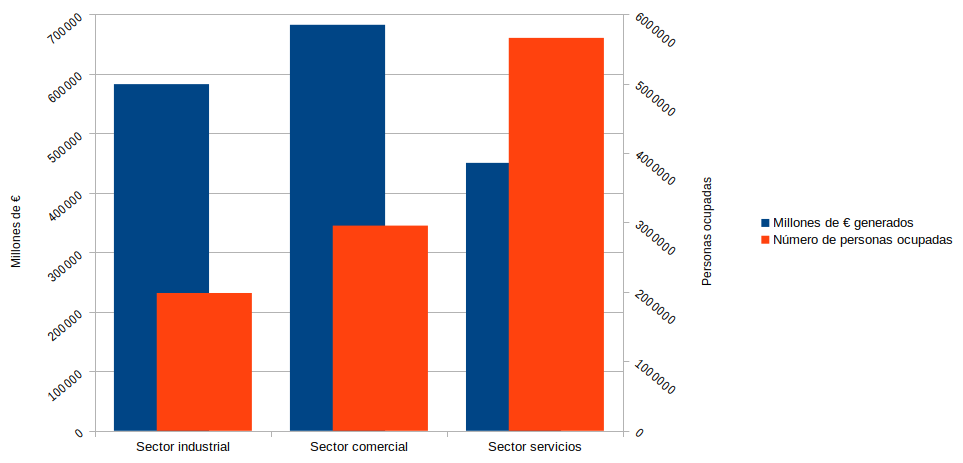
\includegraphics[width=\textwidth]{../graficos/barras_sectores}
  \caption{Distribución de la actividad económica por sectores}
\end{figure}
\end{frame}

\begin{frame}

  Fin.

\end{frame}

\end{document}